\documentclass[11pt, dvipdfmx]{article}
\usepackage{times,deauthor,graphicx}
\usepackage{url}
\usepackage{amssymb}
\usepackage{amsmath}

% algorithm
\usepackage{fancyhdr,amsmath}
\usepackage[ruled,vlined]{algorithm2e}
\usepackage{algorithmic}

%table
\usepackage{booktabs}
\usepackage{multirow}
\usepackage{makecell}
\usepackage{tabularx}


%dashed line
\usepackage{array}
\usepackage{arydshln}
\setlength\dashlinedash{0.2pt}
\setlength\dashlinegap{1.5pt}
\setlength\arrayrulewidth{0.3pt}



\begin{document}

\title{Interpretable Attribute-based Action-aware Bandits for Within-Session Personalization in E-commerce}

\author{Xu Liu$^{1}$, Congzhe Su$^{2}$, Amey Barapatre$^{2}$, Xiaoting Zhao$^{2}$, Diane Hu$^{2}$, Chu-Cheng Hsieh$^{2}$, Jingrui He$^{3}$ \\
$^{1}$ Arizona State University, $^{2}$ Etsy Inc.,
$^{3}$ University of Illinois at Urbana-Champaign \\
xliu338@asu.edu, \{csu, abarapatre, xzhao, dhu, chsieh\}@etsy.com, jingrui.he@gmail.com
}
 
 
\maketitle
\begin{abstract}
When shopping online, buyers often express and refine their purchase preferences by exploring different items in the product catalog based on varying \emph{attributes}, such as color, size, shape, and material. As such, it is increasingly important for e-commerce ranking systems to quickly learn a buyer's fine-grained preferences and re-rank items based on their most recent activity within the session. In this paper, we propose an $O$nline $P$ersonalized $A$ttribute-based $R$e-ranker (\emph{OPAR}), a light-weight, within-session personalization approach using multi-arm bandits (MAB). As the buyer continues on their shopping mission and interacts with different products in an online shop, \emph{OPAR} learns which attributes the buyer likes and dislikes, forming an interpretable user preference profile and improving re-ranking performance over time, within the same session. By representing each arm in the MAB as an attribute, we reduce the complexity space (compared with modeling preferences at the item level) while offering more fine-grained personalization  (compared with modeling preferences at the product category level). We naturally extend this formulation to weight attributes differently in the reward function, depending on how the buyer interacts with the item (e.g. click, add-to-cart, purchase). We train and evaluate \emph{OPAR} on a real-world e-commerce search ranking system and benchmark it against 4 state-of-the-art baselines on 8 datasets and show an improvement in ranking performance across all tasks. 
\end{abstract}


\section{Introduction}\label{sec:intro}
When buyers shop online, they are often faced with thousands, if not millions, of products to explore and potentially purchase. In recent years, we've seen a growing interest in industrial applications of ranking systems as they help minimize distractions for the buyer and surface a digestible number of products that are most relevant to their shopping mission. These ranking systems take the form of search or recommendation systems, where products are ranked in descending order of relevance to the buyer 
\cite{KDD18_TaobaoSearch_RL,KDD18_JD_nextItemRecs,kdd19_amazon_product_search,wu2018turning,MLKD19_JD_onlineRanking,kdd20_sequentialRec}. 

Just as a shopper might browse the aisles of a shop, online shoppers also spend time on a retailer's website searching and clicking on items before they decide what they want to buy. This process is an attempt to refine their purchase intent as they learn more about the product catalog. For example, a buyer might be interested in purchasing a ring; however, they often must click on a number of different rings before they understand possible styles, shapes, colors, and materials that are available. Eventually, the buyer might decide that they have a preference for an emerald gemstone, with a circular shape, and a gold band. Shifting to looking for a necklace, the buyer must refine their preference again.
Often the buyer's preference for attributes like colors and materials changes quickly over the course of one visit. An intelligent ranking system must continually serve content 
that stays relevant to the buyer's changing preference, a capability we refer to as \textit{within-session personalization}. 

Many production ranking systems today have multiple goals to balance: online retailers not only surface content that is \emph{relevant} to the shopper's buying mission (for example, a search query for ``wristwatc" must produce wrist watches), but they also aim show content that is likely to improve a business metric (eg. conversion rate, or GMV). In order to balance these goals, many production ranking systems leverage a 2-stage ranking process (Figure~\ref{fig:ranking_system}): the first pass (commonly referred to as \emph{candidate set selection}) narrows hundreds of millions of items from the product catalog down to a few hundred relevant items \cite{kdd20_facebook_search,kdd19_amazon_product_search, elnlp2020_itemInteraction}; the second pass then re-ranks the top few hundred relevant items in a way that optimizes for specific user action (such as a click or purchase) \cite{guo2020debiasing,kdd20_DNN_airbnb_search,pobrotyn2020contextaware,wu2018turning}. In order to maximize prediction accuracy, these systems often train on billions of historical data points that may span over the course of months or years and thus cannot react quickly enough to the buyer's changing preference within a shopping visit. 

\begin{figure}[!t]
    \centering
    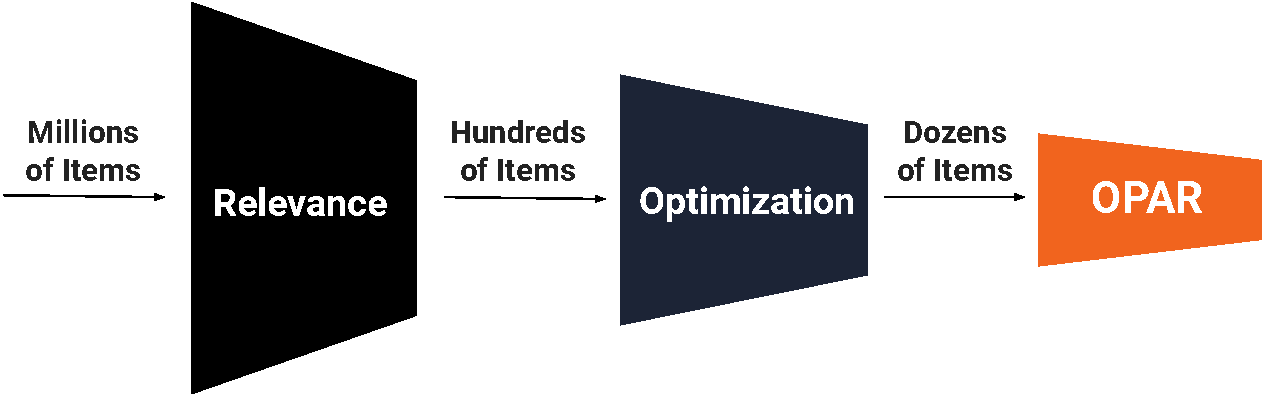
\includegraphics[width=0.645\textwidth]{figs/fig_ranking_system2.pdf}
    \caption{The first two components show a typical 2-stage ranker, where the first-pass narrows down the product catalog to relevant items, while the second-pass performs fine-grained re-ranking to optimize for a business metric. The proposed model, \emph{OPAR}, is responsible for within-session, online personalization that can be effective on its own or as a third-pass ranker on top of a 2-stage ranking system.
    }
    \label{fig:ranking_system}
\end{figure}


In this paper, we propose an $O$nline $P$ersonalized $A$ttribute-based $R$e-ranker (\emph{OPAR}) that can respond quickly to the changing preferences of a buyer within their immediate shopping session, while still reaping the benefits of a traditional 2-stage system. In the MAB literature, it is common to address this problem by treating each arm in the bandit to represent a single item \cite{kdd20_sequentialRec}, product category \cite{recsys16_amazon,MLKD19_JD_onlineRanking} or a context  \cite{KDD18_TaobaoSearch_RL, li2017contextaware,ICML16_contextCascadingBandits}. In contrast, \emph{OPAR} decomposes each product into a descriptive set of attributes (such as its color, texture, material, and shape), and represents each arm as an \emph{attribute}. As the buyer interacts with different products in an online shop, the bandit learns which attributes the buyer likes and dislikes, forming an interpretable user preference profile that is used to re-rank products in real-time in a personalized manner. By representing each arm as an attribute, we reduce the complexity of the space, while allowing more fine-grained personalization within a product category. We naturally extend this formulation to weight attributes differently in the reward function, depending on how the user interacts with that item (e.g. attributes from a clicked item will be weighted less than attributes from an add-to-cart item). 


\begin{figure}[!h]
    \centering
    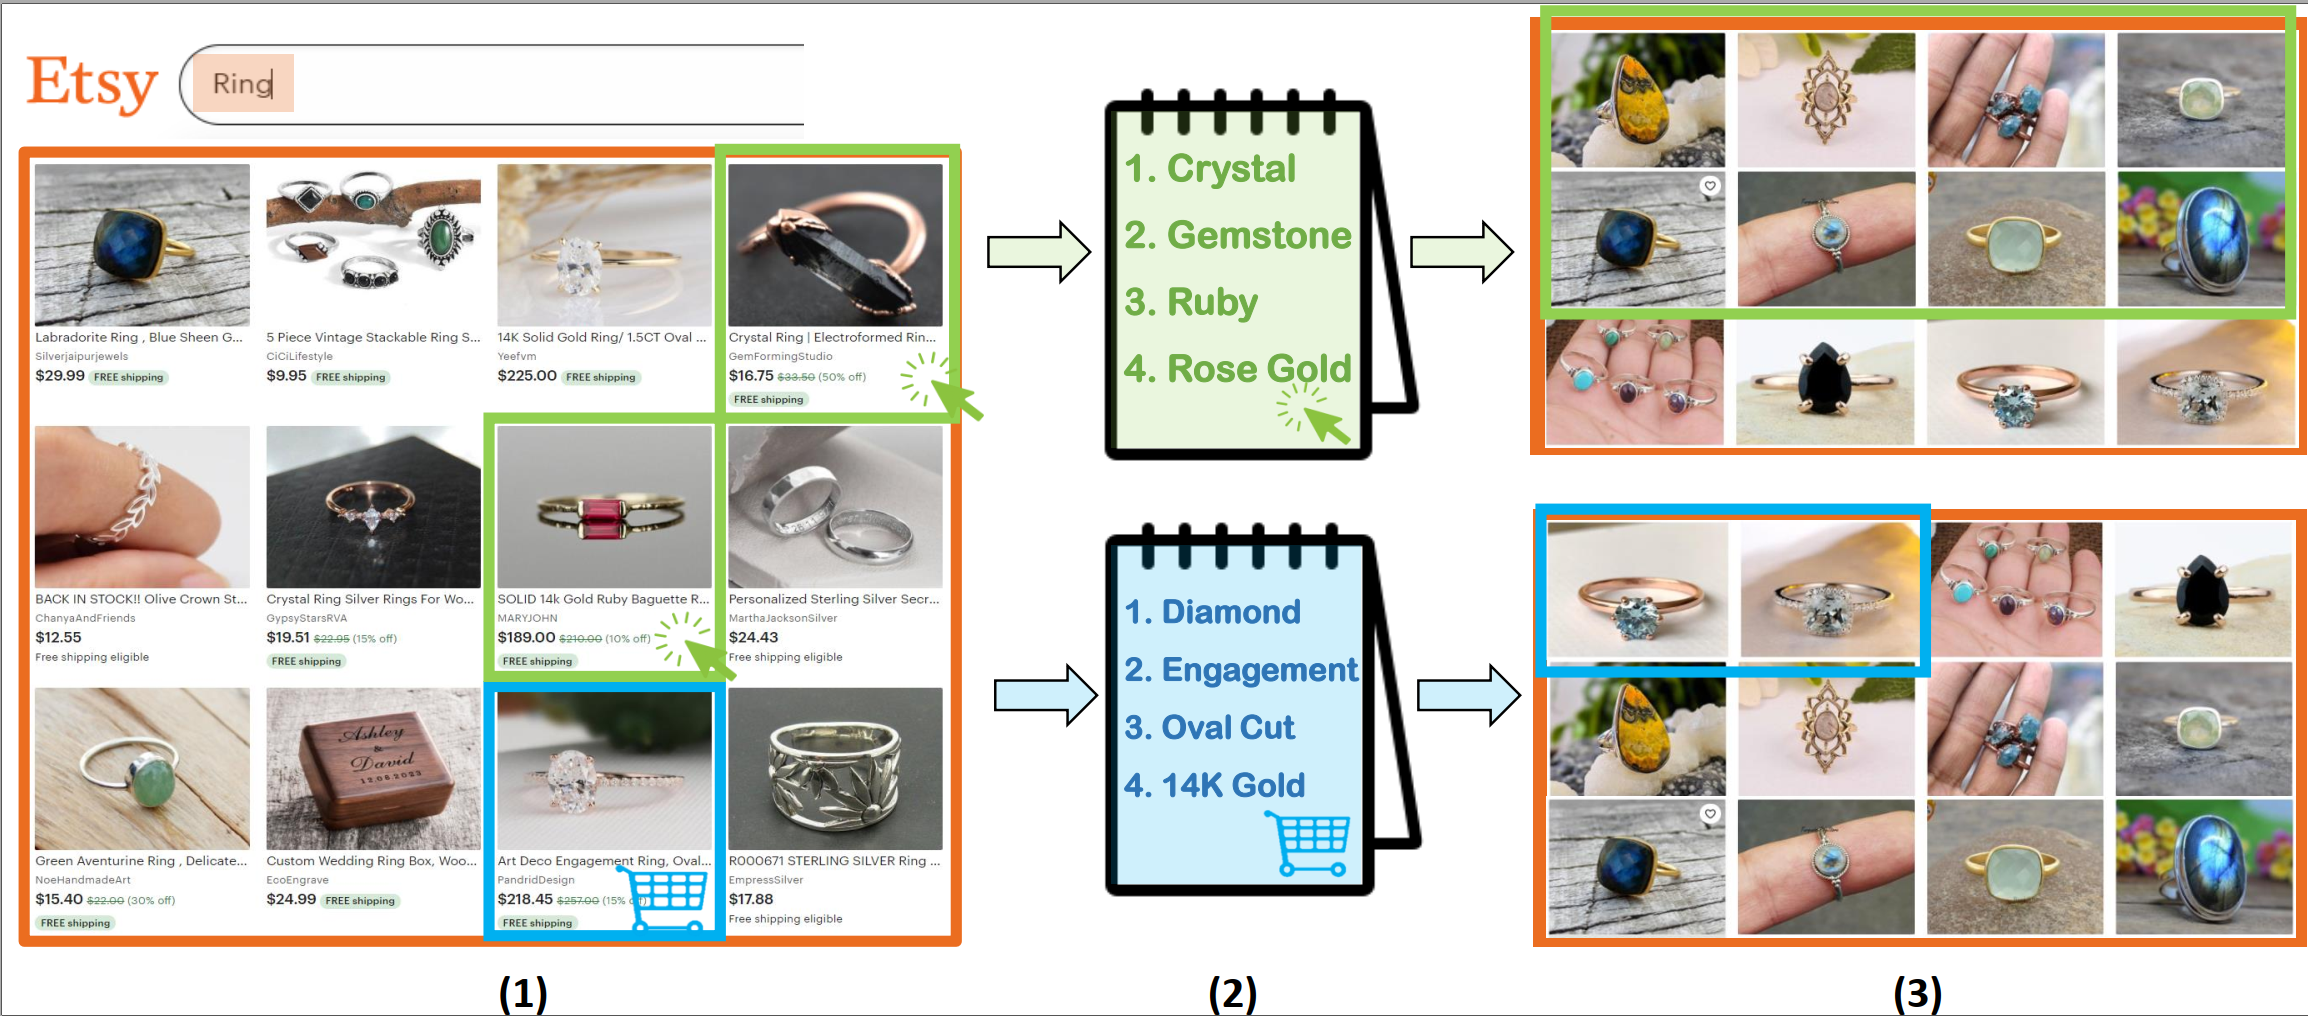
\includegraphics[bb=-145 0 145 100]{figs/fig_toy-cropped_png}
    \caption{Example of attribute and action-aware re-ranking by \emph{OPAR}. From left to right: (1) shows search results for the query ``Ring''. User 1 clicked on two gemstone rings (outlined in green), while User 2 adds a diamond ring to their cart (outlined in blue) (2) The attribute of the clicked items are ``Crystal'', ``Gemstone'', ``Ruby'' and ``Rose Gold'', while the add-to-cart item has the attributes ``Diamond'', ``Engagement'', ``Oval-Cut'' and ``14k Gold'' (3) On a subsequent search page, \emph{OPAR} re-ranks items based on each user's diverging preferences.}
\label{fig:toy}
\end{figure}

In our example of searching for a ring, we see in Figure~\ref{fig:toy} that initially, the same 12 items are shown to two different users. While user 1 might click on items that contain the attributes \emph{crystal, gemstone, ruby,  rose gold} (outlined in \emph{green}), user 2 might have different preferences and click on items that contain the attributes \emph{diamond, engagement, oval cut, 14K gold} (outlined in blue).  At this point, \emph{OPAR} will begin to differentiate the diverging preferences of these two users based on the different attributes that each user has shown interest in. On a subsequent search page, \emph{OPAR} will rank gemstone rings higher for user 1, while user 2 will see diamond rings at the top of the list.  
Furthermore, because the learned weights of each attribute can be observed for each user, our model is extremely interpretable. 

While \emph{OPAR} can be used as a stand-alone algorithm, we find it to be most effective when deployed as a third-pass ranker on top of a traditional two-stage ranking system (see Figure~\ref{fig:ranking_system}). This allows us to leverage the power of traditional 2-pass systems that learn from long-term data aggregated over billions of user and item preferences, while still being nimble enough to personalize a buyer's experience by taking into account their most recent activity. 

In the following, we will introduce the proposed model, \emph{OPAR}, and show how we apply it to a search ranking problem on a popular e-commerce platform. Our contributions are as follows:
\begin{itemize}
    \item \textbf{Attribute-level personalization}: \emph{OPAR} performs real-time personalized re-ranking based on user's preferences at the attribute level and reduces the space complexity while offering more fine-grained personalization. 
    \item \textbf{Light-weight, online re-ranker}: \emph{OPAR} improves ranking performance with little data and requires us to track a minimal number of variables as arms and can be added on top of the traditional 2-pass ranking systems.
    \item \textbf{Interpretable user preferences}: The learned attribute weights give visibility into attributes that the user likes and dislikes. Top-weighted ones can be used for down-stream personalization tasks.
   \item \textbf{Evaluation on real-world datasets}: \emph{OPAR} is trained and evaluated on real-world e-commerce data and is compared to baselines on 8 datasets from a production e-commerce ranking system. We describe a session-level ranking metric to understand ranking improvements within a session.
\end{itemize}


%----------------------------------------------------------------------------------------------------------------------------------------------------------------
%--------------------------------------------------------------        SECTION 2        ---------------------------------------------------------------------
%----------------------------------------------------------------------------------------------------------------------------------------------------------------
\section{Related Work}\label{sec:related_works}
In this section, we summarize the related work from literature and categorize them into two aspects: (1) \textit{Session-based Ranking System}, and (2) \textit{Multi-armed Bandit Ranking System}.
\subsection{Within-Session Ranking}
The within-session ranking task tries to predict what action the user will take next within the current shopping session, leveraging the temporal nature of their browsing behavior from within the same session \cite{KDD18_JD_nextItemRecs, SIGIR16_RNN_nextBasketRec}. Significant breakthroughs in deep learning (i.e, batch normalization and dropout), have led to its wide adoptions in various communities and applications \cite{2019_DNN_rec_survey}. In \cite{Hidasi2016SessionbasedRW}, recurrent neural networks (RNNs) were proposed for this within-session ranking task and gained significant attraction given its superior predictive performance for the next-item recommendation. This has been an active research area with various enhancements proposed specifically for predicting short-term user behavior within the same shopping session \cite{Hidasi2016SessionbasedRW, IJCAI17_sessionContextRecsys,recsys17_sessionRec_perso,DLRS16_sessionBasedRecsys,SIGIR16_RNN_nextBasketRec}.  



Given that a long-term memory models are insufficient to address drift in user interests, \cite{KDD18_STAMP} proposed a short-term attention priority model to capture users' general (long-term) interest in addition to the users' within-session interest via a short-term memory model based on the recent clicks. In parallel, \cite{KDD18_JD_nextItemRecs} studied the behavior-intensive neural network for personalized next-item recommendation by considering both users' long-term preference as well as within-session purchase intent. As RNNs have shown and emerged as the powerful technique to model sequential data for this task, \cite{recsys17_userSesssionIntent} argued for an alternative model, inspired by machine translation, by proposing an encoder-decoder neural architecture with an attention mechanism added to capture user session intents and inter session dependencies. In addition to sequential models, \cite{CIKM19_sessionRec_graphNN} leverages graph neural networks by constructing a session graph and then modeling a weighted attention layer when predicting user's preference in session. To tackle uncertainty that arises in a user's within-session behavior, authors in \cite{KDD19_streaming_sessionRecs} proposed a Matrix Factorization-based attention model to address large-volume and high-velocity session streaming data and \cite{liu2019convolution} handles the missing value issue for the matrix factorization.

Most previous work cited above do not aim for interpretability of its results. In contrast, the model we propose specifically leverages item attributes from the product catalog, resulting in a simple algorithm that learns interpretable user profiles that aid in within-session personalization. The closest related work is \cite{sigir18_nextBucketRec} that proposes the attribute-aware neural attentive model for the next shopping basket recommendation but does not seem to easily adapt for the real-time scenario due to its complexity.   
\vspace{-0.2cm}
\subsection{Multi-Armed Bandits Ranking System}
Requiring a responsive and scalable ranking system that can adapt to the dynamic nature of shifting user preferences (especially in the cold start setting) has led to increasingly wider industry adoption of multi-armed bandit (MAB) in modern day ranking systems. The theoretical foundation and analysis of MABs  have been well-studied, with popular approaches include $\epsilon$-greedy \cite{sutton2018reinforcement}, Upper Confidence Bounds \cite{Auer2002FinitetimeAO}, Thompson sampling \cite{NIPS2011_TS}, EXP3 \cite{Auer2003EXP3}, and others \cite{sutton2018reinforcement}. In the e-commerce \cite{kdd20_sequentialRec} setting, the goal is to maximize user satisfaction (i.e., exploitation), while quickly learning (i.e., exploration) users preferences by exploring unseen content.

Hu et al. in \cite{KDD18_TaobaoSearch_RL} proposed to use reinforcement learning to learn an optimal ranking policy that maximizes the expected accumulative rewards in a search session. 
Yan et al. from \cite{MLKD19_JD_onlineRanking} built a scalable deep online ranking system (DORS) with MABs as the last pass to dynamically re-rank items based on user real-time feedback and showed significant improvement in both users satisfaction and platform revenue. 
Furthermore, authors from \cite{recsys19_interativeRecs} proposed a multi-armed nearest-neighbor bandit to achieve collaborative filtering for the interactive recommendation, by modeling users as arms and exploring the users' neighborhood. \cite{IEEE19_onlineInterativeCF} proposed an interactive collaborative topic regression model that infers the clusters of arms via topic models \cite{LDA} and then utilizes dependent arms for the recommendation. 

In this literature, it is common to address this problem by treating each arm in the bandit to represent a single item \cite{kdd20_sequentialRec}, product category \cite{MLKD19_JD_onlineRanking} or a context  \cite{KDD18_TaobaoSearch_RL,li2017contextaware,ICML16_contextCascadingBandits}. In contrast, \emph{OPAR} decomposes each product into its descriptive set of attributes (such as its color, texture, material, and shape), represents each arm as an \emph{attribute} and provides great explainability in addition to its performance. 

\begin{figure}
    \centering
    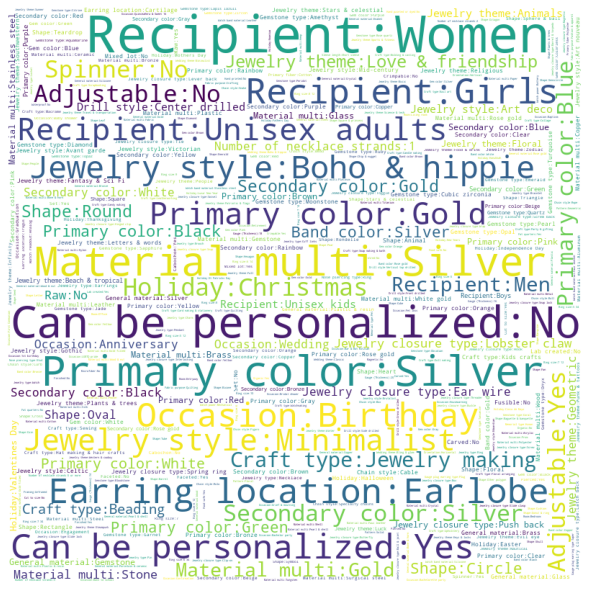
\includegraphics[bb=-220 0 -110 100]{figs/jewelry.png}
    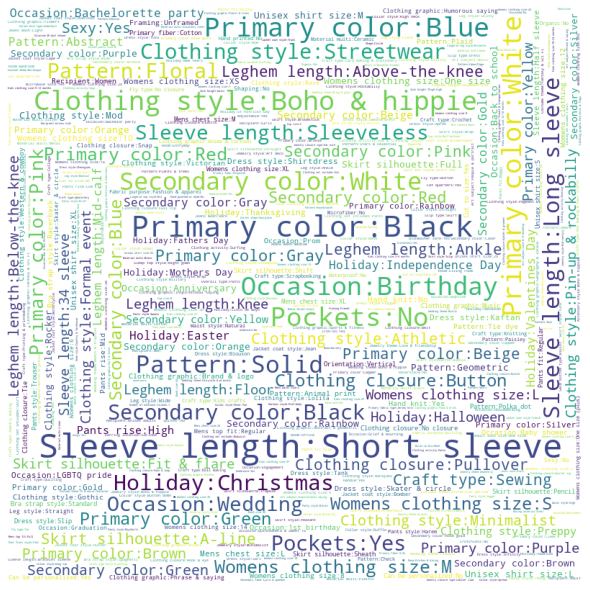
\includegraphics[bb=-110 0 0 100]{figs/clothing.png}
    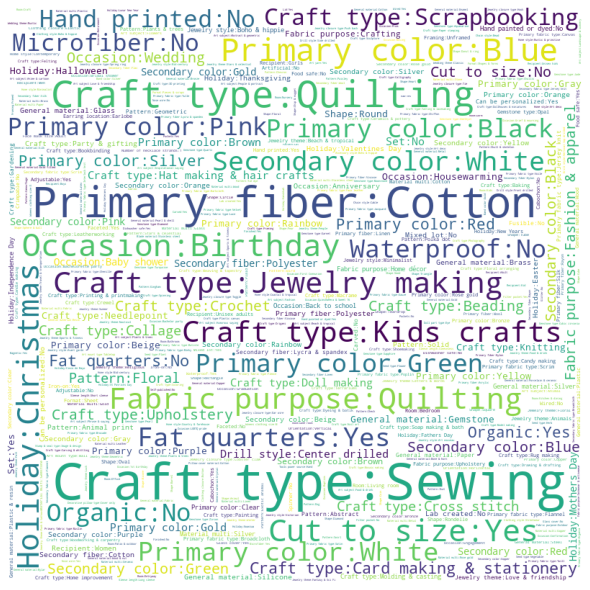
\includegraphics[bb=0 0 110 100]{figs/craft_supplies_and_tools.png}
    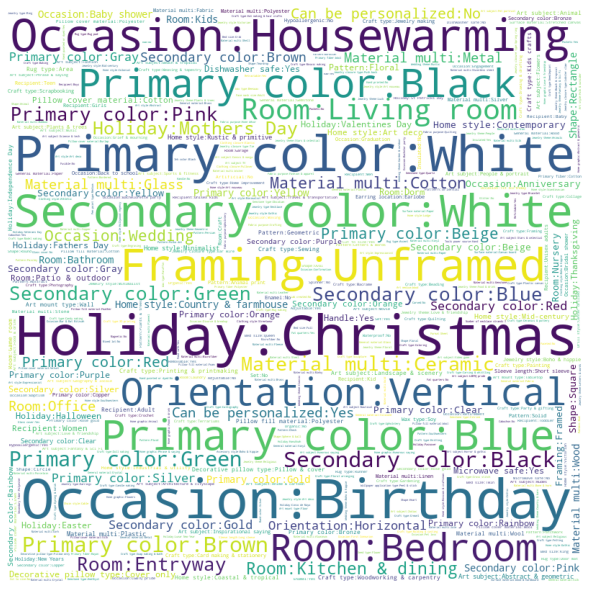
\includegraphics[bb=110 0 220 100]{figs/home_and_living.png}
\caption[Word clouds of item attributes in each dataset]{Top attribute-value pairs for top categories: (1) Jewelry; (2) Clothing; (3) Craft Supplies and Tools, (4) Home and Living.}
\label{fig:wordCloud}
\end{figure}


%----------------------------------------------------------------------------------------------------------------------------------------------------------------
%--------------------------------------------------------------        SECTION 3        ---------------------------------------------------------------------
%----------------------------------------------------------------------------------------------------------------------------------------------------------------
\section{Problem Formulation} \label{sec:problem_formulation}
In this section, we provide definitions for commonly used terms such as sessions and attributes. We then explain our model in two parts: (1) how to represent within-session attribute preferences, and (2) how to re-rank items based on these preferences. 
\subsection{Definitions}
\noindent\textbf{Definition 1: A \textit{session}} is a sequence of  actions that the buyer takes while engaging with an e-commerce platform in trying to fulfill a shopping mission (e.g. search, click, add-to-cart). The session typically ends when the buyer leaves the site with a purchase or abandons after a significant duration of inactivity (e.g., 30 minutes). 
Note that we focus on product search here but should be generally applicable to other ranking or recommendation problems.

Let us define a session $S=\{{[Q_t, I_t, A_t]}\}_{t=1}^T$ that is a sequence of $T$ user actions within a session, in which $T$ can vary across sessions. The session starts at $t=1$ and ends at $T$ with a purchase (or becomes inactive). At each time step, item list $I_t\in R^{M\times 1}$ contains $M$ candidate items to be re-ranked for query $Q_t$, and then how the user engages with the list of items is represented by $A_t$:
\begin{equation}
A_t(x_i)=
\left\{
    \begin{array}{ll}
    0,\,\,\mbox{no action on $x_i$} \\
    1,\,\,x_i\mbox{ is purchased} \\
    2,\,\,x_i\mbox{ is added to cart} \\
    3,\,\,x_i\mbox{ is clicked}
    \end{array}
\right.
, \forall x_i\in I_t.
\label{eq:action_on_item}
\end{equation}

\noindent\textbf{Definition 2: An \textit{attribute}} is a basic unit (e.g. size, color) that describes the product characteristics of an item. The attributes are determined by taxonomists based on the product category while the value of the attributes (e.g. large, green) are volunteered by the seller, or inferred by machine-learned classifiers. 
These attribute-value pairs help buyers efficiently navigate through an overwhelmingly large inventory. Thus, each item $x_i$ is represented as the composition of its attributes, with $H_{x_i}$ denoting the total number of attributes associated with $x_i: x_i=\{atr_1,atr_2,\dots,atr_{H_{x_i}}\}.$

Figure \ref{fig:wordCloud} shows four category-specific word clouds of attributes-value pairs exhibited in items from top categories at Etsy, one of the largest e-commerce platform for handmade, vintage, and craft supplies. Some of the most common attributes are universal: 
size, color, and material. Others are category specific: sleeve length, earring location, and craft type. Lastly, some attributes (e.g. holiday, occasion, recipient) describe how or when the item can be used. 


\subsection{Problem Statement}
Our goal is to (1) formulate each user's within-session preference for product attributes and (2) re-rank a list of candidate items based on the user's inferred within-session preference on item attributes.

\noindent \textbf{Part 1: \textit{How to formulate users' in-session attribute preferences?}}\\
\noindent \textbf{Input}: For session $S$, (1) item lists $\{I_t\}_{t=1}^T$ with each item $x_i=\{atr_{H_{x_i}}\}$ as composition of product attributes; and (2) session-level record of user actions on shown items, $\{A_t\}_{t=1}^T$. \\
\noindent \textbf{Output} User's preference $\mathbf{\Theta}$ on attributes as beta-distributed:  $\mathbf{\Theta}=\{\theta_{atr_n}\}_{n=1}^N \sim \{Beta(\alpha_{atr_n},\beta_{atr_n})\}_{n=1}^N$, where $N$ denotes the total number of attributes encountered in session $S$. 

For a user, we model their within-session preference on an attribute as a latent value $\theta_{atr_n} \in [0,1]$ denoting the probability that they would like the attribute exhibited in the item. 
Motivated by Thompson Sampling \cite{agrawal2012analysis}, let $\theta_{atr_n}$ be beta-distributed, with $\alpha_{atr_n}, \beta_{atr_n}$ be the two parameters of the distribution. In Section \ref{subsec:experimental_setup} we show a method on estimating the parameters of attributes from historical data. From the list of shown items $I_t$, the user engages on a subset of items (denoted in $A_t$) to express their preference for item attributes according to $\mathbf{\Theta}$. Given the feedback, we propagate rewards from the user actions to the associated attributes with increments, $\delta_{A_t(x_i)}$, and update the posterior distribution of $\mathbf{\Theta}$, with rewards normalized at $x_i$ by its cardinality (number of associated attributes on that item). 

\noindent\textbf{Part 2: \textit{How to sequentially re-rank $I_{t}$ based on user preference $\mathbf{\Theta}$} to optimize in-session personalization?} \\
\noindent \textbf{Input}: At time $t$, (1) Candidate list of items $I_t$, and (2) user in-session preference $\mathbf{\Theta}$.\\
\noindent \textbf{Output}: Sequentially learn  $f_t: I_t \times \mathbf{\Theta} \rightarrow \Tilde{I}_t$.

Below we will present the \emph{OPAR} algorithm to address the problem statement discussed here. 




%----------------------------------------------------------------------------------------------------------------------------------------------------------------
%--------------------------------------------------------------        SECTION 4        ---------------------------------------------------------------------
%----------------------------------------------------------------------------------------------------------------------------------------------------------------
\section{Proposed Algorithm, \textit{OPAR}}\label{sec:model}
In this section, we present the details of the proposed \textit{OPAR} model and its extension $\textit{OPAR}_w$ which differentiates different  user actions. 


\begin{algorithm}[!t]
\SetAlgoLined
\KwIn
{\, \\
    \quad Given a session $S=\{{[Q_t, I_t, A_t]}\}_{t=1}^T$ \\ 
    \quad $\{\delta_i\}_{i: \text{ actions}}$: action-aware increments on attribute parameters\\
    \quad $\gamma$: hyper-parameter to control intensity on negatives \\
    \quad $\mathcal{U}_t$, $\mathcal{V}_t$: the associated attributes from engaged items; the associated attributes from impressed items \\
    \quad $|\cdot|_0$: cardinality operator\\
}
\For{$[Q_t, I_t, A_t]\in S$}
{
    \textbf{\textit{(1) Rerank on the Item List $f: I_{t}\rightarrow \Tilde{I}_t$}} \\
    \quad \text{sample }$s_{atr_h}\sim 
         Beta(\alpha_{atr_h},\beta_{atr_h})$, $\forall atr_h \in N_S$ \\
         
    \For{$x_i\in I_{t}$}
    {
        Given $x_i=\{atr_h\}_{h=1}^{H_{x_i}}$ \text{ as associated attributes in } $x_i$, set
        $score(x_i)=\sum_{atr_h \in x_i} g(s_{atr_h})$
    }
    $\Tilde{I}_{t}=sorted([score(x_i)]_{x_i\in I_{t}})$ \\
        \textbf{\textit{(2) Update attribute parameters given $A_t$}}\\
    Let $\mathcal{U}_t = \cup \{atr_h: \forall atr_h\in x_i\,if\,A_t(x_i) \neq 0,\,\forall x_i\in I_t\}$ \\
    Let $\mathcal{ V}_t = \cup \{atr_h: \forall atr_h\in x_i\, \forall x_i\in I_t\}$ \\
    \For{$x_i\in I_t$} 
    {
        \uIf{$A_t(x_i)\neq 0$, item $x_i$ has positive actions }
        {
            $\alpha_{atr_h}+=\delta_{A_t(x_i)}\times \left\{1-Exp\left(-{|\mathcal{U}_t|_0}\right)\right\}$, $\forall atr_h \in x_i$
        }
        \uElseIf{$A_t(x_i)=0$, no action on item $x_i$}
        {
            $\beta_{atr_h}+= \delta_{A_t(x_i)}\times \left\{1-Exp\left(-\gamma{|\mathcal{V}_t\backslash \mathcal{U}_t|_0}\right)\right\}$, $\forall atr_h \in x_i$
        }
        {\textbf{end}}
    }
}
\KwOut{All re-ranking results $[\Tilde{I}_{t}]_{t=1}^{T}$}
\caption{OPAR Algo: Re-Ranking \& Parameter Update}
\label{alg:update}
\end{algorithm}


\subsection{Scoring and Re-ranking Item List}\label{subsec:score_and_rank}
Given attribute-level bandits with each arm as an item attribute, we describe below our approach on how we score and re-rank items, motivated by the Thompson Sampling approach on \cite{agrawal2012analysis}. 

Let $N$ denote the number of attributes associated with item list $I_{t}$. For each attribute in $\{atr_h: atr_h \in x_i,\,\forall x_i\in I_{t}\}$, we randomly sample $\theta_{atr_h}$ from its corresponding distribution, denoting the probability that the user is interested in the attribute, $atr_h$, at time $t$: 
\begin{equation}\label{eq:attribute_sampling}
\centering
    \theta_{atr_h}\sim Beta (\alpha_{atr_h},\beta_{atr_h}).
\end{equation}
Then, each item $x_i\in I_{t}$ is scored and ranked by:
\begin{equation}\label{eq:scoring}
    score(x_i) = \sum_{atr_h \in x_i} g(\theta_{atr_h}),
    \vspace{-0.1cm}
\end{equation}
where $g(\theta_{atr_h})=\frac{1}{rank(\theta_{atr_h})}$ is a harnomic function of the index that $\theta_{atr_h}$ is ranked among $[\theta_{atr_h}]^{H_{x_i}}_{h=1}$, with a tie-breaker uniformly at random. A larger $score(x_i)$ indicates higher satisfication with item $x_i$ given users' short in-session preference on the attributes. Lastly, we present the user $\Tilde{I}_t$, which is reranked list of the items based on $[score(x_i)]_{x_i\in I_{t}}$. 


\subsection{Attribute Parameter Updates}\label{subsec:update_parameters}
With the feedback gathered from the user action $A_t$, we do the following updates for the attribute parameters. Let $\mathcal{U}_t$ denote the set of attributes associated from items with positive actions (i.e., click, add-to-cart, purchase), and $\mathcal{V}_t$ be union of all attributes exist in $x_i \in I_t$: 
\begin{equation*}
\vspace{-0.2cm}
\begin{split}
\centering
\mathcal{U}_t = \cup \{atr_h: \forall atr_h\in x_i\,\text{if}\,A_t(x_i) \neq 0,\,\forall x_i\in I_t\}, \text{  }
\mathcal{ V}_t = \cup \{atr_h: \forall atr_h\in x_i,\, \forall x_i\in I_t\}.
\vspace{-0.3cm}
\end{split}
\end{equation*}
For a given $atr_h$, let $\Tilde{\mathcal{Y}}_{t, atr_h}$ and $\Tilde{\mathcal{Z}}_{t, atr_h}$ denote the set of items associated with positive user action and no-action, respectively,
\begin{equation*}
\begin{split}
\centering
\Tilde{\mathcal{Y}}_{t, atr_h} = \{x_i \in I_t: atr_h \in x_i \text{ and } atr_h \in \mathcal{U}_t\}, \textmd{  }
\Tilde{\mathcal{Z}}_{t, atr_h} = \{x_i \in I_t: atr_h \in x_i \text{ and } atr_h \in \mathcal{V}_t \backslash \mathcal{U}_t\}.
\end{split}
\vspace{-0.3cm}
\end{equation*}

Then, the Beta distribution of each attribute is updated as follows:
\begin{equation}
\label{eq:updating}
\begin{split}
    \alpha_{atr_h} &+= \sum_{\Tilde{\mathcal{Y}}_{t, atr_h}} \delta_{A_t(x_i)} \left(1-e^{-|\mathcal{U}_t|_0}\right), \forall atr_h \in \mathcal{U}_t, \\
    \beta_{atr_h} &+= \sum_{\Tilde{\mathcal{Z}}_{t, atr_h}} \delta_{A_t(x_i)}  \left(1-e^{-\gamma|\mathcal{V}_t \backslash \mathcal{U}_t|_0}\right), \forall atr_h \in \mathcal{V}_t \backslash \mathcal{U}_t,
\end{split}
\vspace{-0.3cm}
\end{equation}
where $|\cdot|_0$ denotes the cardinality operator and $\gamma$ controls intensity on implicit no-actions. 


\subsection{\textit{OPAR} algorithm Procedure}
In summary, given a session $S=\{{[Q_t, I_t, A_t]}\}_{t=1}^T$, \emph{OPAR} can be summarized with the following steps, with the pseudo code of $\textit{OPAR}_w$ shown in Algorithm \ref{alg:update}. 
\begin{enumerate}
    \item Initialize attribute dictionary $atrDic\in R^{N\times 2}$, which contains $N$ pairs of parameters for attributes, where each row of $atrDic$ denotes the Beta distribution parameter set $(\alpha_{atr}, \beta_{atr})$ for a given attribute. Different initializations have been experimented, including uniform, random or estimated based on held-out historical datasets (shown in Section \ref{subsec:experimental_setup}).  
    \item At time $t$, we score each item $x_i\in I_{t}$ based on Eq. (\ref{eq:scoring}): it first aggregates over the associated attribute preferences sampled in Eq. (\ref{eq:attribute_sampling}), and then re-rank items based on scores in Eq. (\ref{eq:scoring}) and present as $\Tilde{I}_t$. More details in Section \ref{subsec:score_and_rank}.
    \item At time $t$, we receive the obervation $A_t$ on $I_t$, and then update the distribution of all attributes associated with item $x_i$ in the \textit{atrDic} based on the Eq. (\ref{eq:updating}) described in Section \ref{subsec:update_parameters}. 
    
    \textbf{OPAR}: attribute-based bandits with \textit{equal} action-weighting for actions in $\{\text{click}, \text{add-to-cart}, \text{purchase}\}$. This means that for positive actions,
    $\delta_{\text{click}} = \delta_{\text{add-to-cart}}=\delta_{\text{purchase}}$.
    
    $\textbf{OPAR}_w$: extend \textit{OPAR} to weight action-aware updates as follows, $\delta_{\text{click}} \neq  \delta_{\text{add-to-cart}} \neq \delta_{\text{purchase}}$, and hypertune them.
    
    \item We iterate step (2) and (3) until the end of the session.   
\end{enumerate}


%----------------------------------------------------------------------------------------------------------------------------------------------------------------
%--------------------------------------------------------------        SECTION 5       ---------------------------------------------------------------------
%----------------------------------------------------------------------------------------------------------------------------------------------------------------
\section{Experiments} \label{sec:experiments}
\begin{table}[!t] 
\centering
\caption{Etsy Real-world Session-based Dataset Over 3 weeks}
\resizebox{\linewidth}{!}{
\begin{tabular}{@{}crccccc@{}}\toprule
\textbf{ID}&\textbf{Category}& \textbf{$|$Session (User)$|$} & \textbf{$|$Query$|$} & \textbf{$|$Item$|$} & \textbf{$|$Attributes$|$} & \textbf{$|$Actions$|$} \\ \midrule
\textbf{1} &\textbf{Clothing}                                       & 4642                & 46091                  & 1100040            & 2495                       & 58932\\ \hdashline
\textbf{2} &\textbf{Home} \& \textbf{Living}                & 9073                & 103959                & 2282542            & 2455                      & 134416 \\ \hdashline
\textbf{3} &\textbf{Paper} \& \textbf{Party Supplies}  & 4419                & 35132                  & 691919              & 1666                       & 55037 \\ \hdashline
\textbf{4} &\textbf{Craft Supplies} \& \textbf{Tools}    & 10913              & 123662                & 2536492            & 2799                       & 171363 \\ \hdashline
\textbf{5} &\textbf{Accessories}                                 & 5813                & 38215                  & 897533              & 2419                       & 49342 \\ \hdashline
\textbf{6} &\textbf{Electronics \& Accessories}          & 1638                & 10505                  & 216860              & 1302                       & 14354\\ \hdashline
\textbf{7} &\textbf{Jewelry}                                        & 5585                & 67507                  & 1530285             & 2266                      & 79874 \\ \hdashline
\textbf{8} &\textbf{Overall Category}                         & 26442               & 474594               & 9295453             & 3363                      & 624882  \\ \hdashline
\bottomrule
\end{tabular}
}
\label{tb:dataset}
\end{table}


In this section, we show how \textit{OPAR} performs on a real-world e-commerce ranking system and benchmark it against 4 baselines on 8 datasets. While \emph{OPAR} can be applied to any content that requires re-ranking, we specifically chose to train, evaluate, and analyze the model performance on a search ranking system, as the explicit search queries issued by a user shows higher purchase intent, allowing us to better evaluate \emph{OPAR}'s ranking and interpretation capabilities. Our experimentation seeks to answer the following questions:\\
\noindent \textbf{Experiment \#1:} What is the ranking performance of the proposed \textit{OPAR} model? \textit{(Answered in subsection \ref{exp1})}\\
\noindent \textbf{Experiment \#2:} How does \textit{OPAR} perform as an action-aware model? \textit{(Answered in subsection \ref{exp3})}\\
\noindent \textbf{Experiment \#3:} How does \textit{OPAR} help to understand users' short-term, in-session shopping preference? \textit{(Answered in subsection \ref{exp4})}


\subsection{Data Collection}\label{sec:dataset}
The dataset is collected and sampled from a month of user search logs at Etsy, one of the largest e-commerce platforms for handmade, vintage items, and craft supplies. To avoid bot traffic, 
filters are added to include sessions with at least $10$ search events (i.e., queries, browses, clicks, add-to-carts) and at least one \textit{purchase} to focus on sessions with strong shopping missions. Using an existing query classifier, we predict the most probable category (e.g. jewelry, home and living) associated with the first query of each session, and then bucket the entire session into one of 7 categories. This helps us understand shopping behaviors within each category. 
Table \ref{tb:dataset} shows statistics of each data set, representing nearly ~500k search queries from 26k sessions and 620k user actions combined on nearly ten million items, with cardinalities computed within each dataset. We do not perform the evaluation on existing public datasets, because (to the best of our best knowledge) there is no existing dataset that includes all meta-data needed for our study (e.g. query, item attribute, user interaction logs).


\subsection{Experimental Set-up}\label{subsec:experimental_setup}
We split each of the 8 datasets into 2 parts (with sessions ordered chronologically). The first two-thirds of the data is a \textbf{held-out dataset}. Because we are focused on online learning, using only within-session data, the held-out dataset is mainly used for estimating the parameters of the Beta distributions, $\{(\alpha_{atr}, \beta_{atr})\}_{\forall atr}$, and to aggregate attribute counts associated with engaged items to determine attribute popularity, powering the ``Atr-POP'' algorithm in Section \ref{sec:metrics_and_baselines}. 
The remaining data is the \textbf{testing dataset}, on which we report re-ranking performance for \emph{OPAR} and other baseline algorithms on in Table \ref{result:allComparison}. 

While \emph{OPAR} can function as a stand-alone ranking algorithm, we evaluate OPAR (as well as other baselines) on top of an existing 2-pass ranking system (as described in Figure~\ref{fig:ranking_system}). More formally, each session in the testing dataset, $S=\{{[Q_t, I_t, A_t]}\}_{t=1}^T$ contains a sequential list of query content $Q_t$, a candidate set $I_t$ of items to be re-ranked, and logged user actions $A_t$ on $I_t$ (e.g. click, purchase). In our experiments, $I_t$ is a truncated list of the top $48$ items returned by an existing 2-pass ranker, indicating that this list comprises of the most relevant items to the query. As we will see in experimental results, applying \emph{OPAR} adds an effective layer of attribute-based personalization in real-time that was not feasible with the underlying system. In order to simulate an online environment, only within-session user interactions leading up to the current time step are used for ranking predictions. 


\subsection{Evaluation Metrics and Baselines}\label{sec:metrics_and_baselines}
Below, we describe the offline metrics we use to evaluate \emph{OPAR} on the testing dataset, as well as the baselines we benchmark. 

\subsubsection{Evaluation Metrics} Following the general ranking metric Normalized Discounted Cumulative Gain (NDCG) \cite{wang2013theoretical}, we propose a set of session-level ranking metrics to evaluate our model.
\begin{enumerate}
    \item \textit{Click\mbox{-}NDCG}: For each query $Q_t$ issued in $S$ that has at least one click in $A_t$ (i.e, clicks as relevances), $\textit{click-NDCG}_t$ measures the re-ranking performance of the item list $\Tilde{I}_t$ (after re-ranking $I_t$) shown to the user at $t$. For all timestamp with at least a click, we first compute stepwise sequential re-ranking performance $\textit{click\mbox{-}NDCG}_t$ as:
    \begin{equation}
        click\mbox{-}NDCG_t = click\mbox{-}DCG_t / IDCG_t, \forall t=1,...T,
    \end{equation}
    and $\textit{click\mbox{-}NDCG}$ of a session $S$ is the average of $\textit{click\mbox{-}NDCG}_t$ over events that have at least one click: 
    \begin{equation}
        \textit{click\mbox{-}NDCG} = \text{Average}( \textit{click\mbox{-}NDCG}_t).
    \end{equation}
    
    \item \textit{Purchase-NDCG}: Following the above methodology, we compute the session-level re-ranking performance limit to search events with attributed purchases. A session on a shopping site is defined as a sequence of events ending with a purchase or a significant duration of inactivity. Given that, \textit{Purchase\mbox{-}NDCG} given a session is essentially $\textit{purchase\mbox{-}NDCG}_T$. 
\end{enumerate}


For each re-ranking algorithm reported in Table \ref{result:allComparison}, we compute $\textit{Click\mbox{-}NDCG}$ @k and \textit{Purchase\mbox{-}NDCG}@k for $k=\{4,12,24,48\}$ by averaging $\textit{click\mbox{-}NDCG}_s$ @k and $\textit{purchase\mbox{-}NDCG}_s$@k given session $s$ over all sessions in each dataset. Note that $k$ is a multiple of 4 as that this shopping site displays 4 items per row on desktops. 


\begin{table}[t]
\caption{Re-ranking performance comparison on over all data sets (top-left) and 7 category-specific data sets.}
\resizebox{\textwidth}{!}{
\begin{tabular}{ccccccccccccccc}
\toprule
                                                                         &     & \multicolumn{6}{c}{Over All Category}                               &  & \multicolumn{6}{c}{Clothing}                               \\ \cline{3-8} \cline{10-15} 
                                                                         &     & LambdaMART & Atr-KNN & Atr-POP & GRU4Rec & OPAR  & $\text{OPAR}_w$        &  & LambdaMART & Atr-KNN & Atr-POP & GRU4Rec & OPAR  & $\text{OPAR}_w$ \\ \hline
\multirow{4}{*}{\begin{tabular}[c]{@{}c@{}}Purchase\\ NDCG\end{tabular}} & @4  & 0.1795     & 0.0130  & 0.0749  & 0.0618  & 0.2994 & \textbf{0.3042} &  & 0.1948     & 0.0103  & 0.0516  & 0.0551  & 0.2384 & \textbf{0.2494} \\ \cdashline{2-15} 
                                                                         & @12 & 0.2629     & 0.0412  & 0.1323  & 0.1425  & 0.3505 & \textbf{0.3607} &  & 0.2670     & 0.0348  & 0.1269  & 0.0824  & 0.2685 & \textbf{0.2744} \\ \cdashline{2-15} 
                                                                         & @24 & 0.3162     & 0.1260  & 0.2112  & 0.2018  & 0.3718 & \textbf{0.3900} &  & 0.3019     & 0.0090  & 0.2193  & 0.1434  & 0.3209 & \textbf{0.3263} \\ \cdashline{2-15} 
                                                                         & @48 & 0.3724     & 0.2554  & 0.2861  & 0.2518  & 0.4512 & \textbf{0.4578} &  & 0.3774     & 0.2462  & 0.2784  & 0.2157  & 0.3976 & \textbf{0.4030} \\ \hline
\multirow{4}{*}{\begin{tabular}[c]{@{}c@{}}Click\\ NDCG\end{tabular}}    & @4  & 0.1459     & 0.0816  & 0.0705  & 0.0701  & 0.3120 & \textbf{0.3158} &  & 0.1328     & 0.0067  & 0.0690  & 0.0691  & 0.3058 & \textbf{0.3197} \\ \cdashline{2-15} 
                                                                         & @12 & 0.2265     & 0.1456  & 0.1264  & 0.1354  & 0.3213 & \textbf{0.3229} &  & 0.2137     & 0.0228  & 0.1224  & 0.1414  & 0.3126 & \textbf{0.3257} \\ \cdashline{2-15} 
                                                                         & @24 & 0.2955     & 0.2157  & 0.2021  & 0.1922  & 0.3318 & \textbf{0.3489} &  & 0.2821     & 0.0658  & 0.2045  & 0.1844  & 0.3274 & \textbf{0.3424} \\ \cdashline{2-15} 
                                                                         & @48 & 0.3815     & 0.3245  & 0.2813  & 0.2689  & 0.4047 & \textbf{0.4051} &  & 0.3711     & 0.2309  & 0.2807  & 0.2613  & 0.3988 & \textbf{0.4061} \\ \hline \hdashline \hline
                                                                         &     & \multicolumn{6}{c}{Home \& Living}                           &  & \multicolumn{6}{c}{Paper \& Party Supplies}                         \\ \cline{3-8} \cline{10-15} 
                                                                         &     & LambdaMART & Atr-KNN & Atr-POP & GRU4Rec & OPAR  & $\text{OPAR}_w$ &  & LambdaMART & Atr-KNN & Atr-POP & GRU4Rec & OPAR  & $\text{OPAR}_w$ \\ \hline
\multirow{4}{*}{\begin{tabular}[c]{@{}c@{}}Purchase\\ NDCG\end{tabular}} & @4  & 0.1755     & 0.0131  & 0.0649  & 0.0571  & 0.2920 & \textbf{0.2952}   &  & 0.1822     & 0.0010  & 0.1255  & 0.0684  & 0.2828 & \textbf{0.2965} \\ \cdashline{2-15} 
                                                                         & @12 & 0.2670     & 0.0396  & 0.1226  & 0.1281  & 0.3391 & \textbf{0.3436}   &  & 0.2667     & 0.0406  & 0.1692  & 0.0941  & 0.3367 & \textbf{0.3497} \\ \cdashline{2-15} 
                                                                         & @24 & 0.3218     & 0.0936  & 0.2066  & 0.1752  & 0.3838 & \textbf{0.3879}   &  & 0.3276     & 0.1297  & 0.2469  & 0.1542  & 0.3796 & \textbf{0.3905} \\ \cdashline{2-15} 
                                                                         & @48 & 0.3874     & 0.2543  & 0.2789  & 0.2164  & 0.4462 & \textbf{0.4491}   &  & 0.3876     & 0.2550  & 0.3216  & 0.1943  & 0.4291 & \textbf{0.4399} \\ \hline
\multirow{4}{*}{\begin{tabular}[c]{@{}c@{}}Click\\ NDCG\end{tabular}}    & @4  & 0.1481     & 0.0054  & 0.0601  & 0.0944  & 0.3201 & \textbf{0.3219}   &  & 0.1585     & 0.0052  & 0.1084  & 0.0839  & 0.2825 & \textbf{0.2874} \\ \cdashline{2-15} 
                                                                         & @12 & 0.2294     & 0.0213  & 0.1175  & 0.1416  & 0.3244 & \textbf{0.3256}   &  & 0.2394     & 0.0247  & 0.1586  & 0.1367  & 0.2931 & \textbf{0.2973} \\ \cdashline{2-15} 
                                                                         & @24 & 0.2978     & 0.0598  & 0.1973  & 0.1843  & 0.3485 & \textbf{0.3491}   &  & 0.3103     & 0.0644  & 0.2300  & 0.1742  & \textbf{0.3383} & 0.3189 \\ \cdashline{2-15} 
                                                                         & @48 & 0.3835     & 0.2278  & 0.2746  & 0.2288  & 0.4032 & \textbf{0.4086}   &  & 0.3911     & 0.2306  & 0.3104  & 0.2007  & 0.4017 & \textbf{0.4072} \\ \hline \hdashline \hline
                                    &     & \multicolumn{6}{c}{Craft Supplies \& Tools}                         &  & \multicolumn{6}{c}{Accessories}                            \\ \cline{3-8} \cline{10-15} 
                                                                         &     & LambdaMART & Atr-KNN & Atr-POP & GRU4Rec & OPAR  & $\text{OPAR}_w$ &  & LambdaMART & Atr-KNN & Atr-POP & GRU4Rec & OPAR  & $\text{OPAR}_w$ \\ \hline
\multirow{4}{*}{\begin{tabular}[c]{@{}c@{}}Purchase\\ NDCG\end{tabular}} & @4  & 0.1912     & 0.0135  & 0.0739  & 0.0741  & 0.3101 & \textbf{0.3268}   &  & 0.1954     & 0.0251  & 0.0683  & 0.0511  & 0.2166 & \textbf{0.2178} \\ \cdashline{2-15} 
                                                                         & @12 & 0.2735     & 0.0407  & 0.1296  & 0.1125  & 0.3673 & \textbf{0.3781}   &  & 0.2828     & 0.0741  & 0.1431  & 0.0849  & \textbf{0.2835} & 0.2930 \\ \cdashline{2-15} 
                                                                         & @24 & 0.3272     & 0.1208  & 0.1970  & 0.1644  & 0.4084 & \textbf{0.4188}   &  & 0.3324     & 0.1406  & 0.2510  & 0.1222  & 0.3304 & \textbf{0.3361} \\ \cdashline{2-15} 
                                                                         & @48 & 0.3844     & 0.2577  & 0.2820  & 0.2214  & 0.4366 & \textbf{0.4750}   &  & 0.3869     & 0.2693  & 0.2917  & 0.1641  & 0.3962 & \textbf{0.4020} \\ \hline
\multirow{4}{*}{\begin{tabular}[c]{@{}c@{}}Click\\ NDCG\end{tabular}}    & @4  & 0.1458     & 0.0055  & 0.0749  & 0.0994  & 0.3118 & \textbf{0.3166}   &  & 0.1502     & 0.0105  & 0.0673  & 0.0712  & 0.2495 & \textbf{0.2605} \\ \cdashline{2-15} 
                                                                         & @12 & 0.2262     & 0.0513  & 0.1290  & 0.1279  & 0.3241 & \textbf{0.3293}   &  & 0.2324     & 0.0439  & 0.1358  & 0.1331  & 0.2656 & \textbf{0.2708} \\ \cdashline{2-15} 
                                                                         & @24 & 0.2955     & 0.2042  & 0.1953  & 0.1935  & \textbf{0.3525} & 0.3521   &  & 0.3006     & 0.1091  & 0.2398  & 0.1800  & 0.3155 & \textbf{0.3212} \\ \cdashline{2-15} 
                                                                         & @48 & 0.3811     & 0.2278  & 0.2815  & 0.2277  & \textbf{0.4080} & 0.4078   &  & 0.3848     & 0.2391  & 0.2885  & 0.2312  & 0.3548 & \textbf{0.4029} \\ \hline \hdashline \hline
                                                                         &     & \multicolumn{6}{c}{Electronics \& Accessories}                            &  & \multicolumn{6}{c}{Jewelry}                                \\ \cline{3-8} \cline{10-15} 
                                                                         &     & LambdaMART & Atr-KNN & Atr-POP & GRU4Rec & OPAR  & $\text{OPAR}_w$ &  & LambdaMART & Atr-KNN & Atr-POP & GRU4Rec & OPAR  & $\text{OPAR}_w$ \\ \hline
\multirow{4}{*}{\begin{tabular}[c]{@{}c@{}}Purchase\\ NDCG\end{tabular}} & @4  & 0.2136     & 0.0501  & 0.0715  & 0.0814  & 0.2847 & \textbf{0.2995}   &  & 0.1661     & 0.0060  & 0.0576  & 0.0718  & 0.3051 & \textbf{0.3285} \\ \cdashline{2-15} 
                                                                         & @12 & 0.3014     & 0.1109  & 0.1546  & 0.1223  & 0.3386 & \textbf{0.3782}   &  & 0.2534     & 0.0766  & 0.1074  & 0.1142  & 0.3484 & \textbf{0.3854} \\ \cdashline{2-15} 
                                                                         & @24 & 0.3519     & 0.0176  & 0.2652  & 0.1674  & \textbf{0.4257} & 0.4152   &  & 0.3087     & 0.1470  & 0.1668  & 0.1847  & 0.3866 & \textbf{0.3973} \\ \cdashline{2-15} 
                                                                         & @48 & 0.4060     & 0.2965  & 0.2981  & 0.2416  & 0.4516 & \textbf{0.4656}   &  & 0.3814     & 0.2460  & 0.2663  & 0.2367  & 0.4425 & \textbf{0.4598} \\ \hline
\multirow{4}{*}{\begin{tabular}[c]{@{}c@{}}Click\\ NDCG\end{tabular}}    & @4  & 0.1530     & 0.0267  & 0.0805  & 0.0641  & \textbf{0.2074} & 0.2051   &  & 0.0701     & 0.0027  & 0.0621  & 0.0614  & 0.3314 & \textbf{0.3892} \\ \cdashline{2-15} 
                                                                         & @12 & 0.2324     & 0.0703  & 0.1580  & 0.0939  & 0.2487 & \textbf{0.2622}   &  & 0.1314     & 0.0106  & 0.1141  & 0.1021  & 0.3783 & \textbf{0.3963} \\ \cdashline{2-15} 
                                                                         & @24 & 0.3029     & 0.1410  & 0.2657  & 0.1345  & \textbf{0.3158} & 0.3120   &  & 0.1989     & 0.1276  & 0.1762  & 0.1647  & 0.3956 & \textbf{0.4162} \\ \cdashline{2-15} 
                                                                         & @48 & 0.3880     & 0.2560  & 0.3026  & 0.1667  & 0.3978 & \textbf{0.4078}   &  & 0.3119     & 0.2192  & 0.2700  & 0.2144  & 0.4190 & \textbf{0.4475} \\ \bottomrule
\end{tabular}}
\label{result:allComparison}
\end{table}


\subsubsection{Baselines} We compared \textit{OPAR}'s ranking performance with 4 state-of-the-art baselines:
\begin{enumerate}
    \item LambdaMART \cite{wu2010adapting} is the boosted tree version of LambdaRank \cite{burges2007learning}, which introduces the use of gradient boosted decision trees for solving a ranking task and won Track 1 of the 2010 Yahoo! Learning To Rank Challenge. A personalized search re-ranker is trained based on long-term user historical data to optimize for the user's purchasability on an item given the query issued and the user's historical preference. 
    \item Atr-KNN is derived from Item-KNN \cite{Hidasi2016SessionbasedRW}. Each item is presented by n-hot-encoding of associated attributes with $n$ being the cardinality of all attributes. That is, its $i^{th}$ entry equals to 1 if the referred attribute presents in the item, otherwise 0. Items in the list $I_{t+1}$ are re-ranked based on their euclidean-distance from the last engaged item(s) in $I_t$. Note that the items $x_i \in I_t$ with no-action has no impact on this re-ranking.
    \item Atr-POP reranks the candidate set, $I_t$,  of items based on the attributes' popularity estimated with held-out historical records. This baseline is one of the most common solutions derived from \cite{Hidasi2016SessionbasedRW} given its simplicity and efficacy.
    \item GRU4Rec \cite{Hidasi2016SessionbasedRW} applies recurrent neural networks (RNN) on short session-based data of clicked items to achieve session-based next-item recommendation. Each session is encoded as a 1-of-N vector, in which the $i^{th}$ entry is 1 if the corresponding item is clicked else 0, with N denoting the number of items. 
    While the user's consecutive clicks on items are used in the next item prediction, it is attribute-agnostic. 
\end{enumerate}

While it is common for each arm in the bandits to represent a single item or product category, we skip it as a baseline here as this would incur higher exploration cost with potential latency bottleneck when scaling up to an inventory of hundred millions of items and also lose interpretability of product attributes. 


\begin{table*}[!t]
\caption{Multiple Purchase Intents within One Session}
\label{tb:queries}
\resizebox{\textwidth}{!}{
\begin{tabular}{cclcrl}
\toprule
\textbf{}                                                                                 & \textbf{Timestamp} & \multicolumn{1}{c}{\textbf{Query}}  & \textbf{Query Taxonomy}  & \multicolumn{2}{c}{\textbf{Engaged Attributes}}                                                                                                                                                                          \\ \hline \vspace{-3.5mm} \\ \cdashline{2-6} 
\multirow{4}{*}{\textbf{\begin{tabular}[c]{@{}c@{}}\\ \, \\1st\\ Purchase\\ Intent\end{tabular}}} & 0          & 'flower girl basket'                & paper and party supplies & (NO ACTION) & Browsing                                                                                                                                                                                                   \\ \cdashline{2-6} 
                                                                                          & 1-4                & 'flower girl basket wedding'        & paper and party supplies & (CLICK)     & \begin{tabular}[c]{@{}l@{}}'Prime Color: White', 'Occasion: Wedding', 'Holiday: Christmas',\\ 'Wedding theme: Beach $\&$ tropical',  'Craft type: Floral arranging'\end{tabular}                             \\ \cdashline{2-6} 
                                                                                          & 5-9                & 'flower girl basket beach wedding'  & paper and party supplies & (CLICK)     & \begin{tabular}[c]{@{}l@{}}'Prime Color: Blue', 'Occasion: Wedding', 'Holiday: Christmas', \\ 'Wedding theme: Beach $\&$ tropical', 'Secondary color: White', 'Craft type: Floral arranging'\end{tabular} \\ \cdashline{2-6} 
                                                                                          & 10-11              & 'two flower girl and one pillow'    & paper and party supplies &  & Browsing    \\ \cdashline{2-6} \vspace{-3mm} \\ \hline      
\multicolumn{6}{c}{\textbf{Purchase Intent Change}}                                                                                                                                                                                                                                                                                                                                                        \\ \hline \vspace{-3mm} \\ \cdashline{2-6}
\multirow{3}{*}{\textbf{\begin{tabular}[c]{@{}c@{}}2nd\\ Purchase\\ Intent\end{tabular}}} & 12-15              & 'hat for beach wedding'             & clothing.women\_clothing & (CLICK)     & 'Prime Color: Blue', 'Occasion: Wedding'                                                                                                                                                                   \\ \cdashline{2-6} 
                                                                                          & 16-22              & 'turquoise petals'                  & accesories               & (CLICK)     & \begin{tabular}[c]{@{}l@{}}'Prime Color: Blue', 'occasion: Bridal shower', 'Wedding theme: Fairytale $\&$ princess'\end{tabular}                                                                         \\ \cdashline{2-6} 
                                                                                          & 23                 & 'bride hair decoration beach theme' & clothing.women\_clothing & (NO ACTION) & Browsing              \\ \cdashline{2-6} \vspace{-3.5mm}                                                                                                                                                   \\ \hline \vspace{-3mm} \\ \cdashline{2-6}
\multirow{2}{*}{\textbf{\begin{tabular}[c]{@{}c@{}}Final Purchase\end{tabular}}}          & 24                 & 'turquoise petals'                  & accesories              & (PURCHASE) & \begin{tabular}[c]{@{}l@{}}'Prime Color: Blue', 'Occasion: Bridal shower',  'Wedding theme: Fairytale $\&$ princess'\end{tabular} \\ \bottomrule                                                                                        
\end{tabular}
}
\end{table*}


\subsection{Experimental Results}
In this section, we describe experimentation results for evaluating three kinds of performance: (1) ranking performance, (2) impact of differentiating between user action types, and (3) interpretability.


\subsubsection{Overall Re-ranking Performance}\, \label{exp1} 
\noindent Table \ref{result:allComparison} shows experiment results of our model (\textit{OPARs}) against 4 baselines described in Section \ref{sec:metrics_and_baselines}. The results can be categorized into two parts: (1) performance on the aggregated datasets over all categories (top-left); and (2) performance on each of the 7 category-specific datasets, representing different shopping missions and behaviors across categories (i.e, ``Clothing'', ``Home $\&$ Living''). Across all 8 datasets for the re-ranking task, $\textit{OPAR}_w$ 
outperform against all 4 baselines, including LambdaMART, Atr-KNN, Atr-POP, and GRU4Rec in both purchase-NDCG and click-NDCG. 

For the overall dataset (top-left), $\textit{OPAR}_w$ shows over $6\%$ lift in click-NDCG@48 compared to the best baseline, and over 20\% increase in purchase-NDCG@48. Similar results are observed in each category-specific re-ranking. For $k$, the best improvement for $\textit{OPAR}_w$ is achived at $k=4$, ordering by $@4>>@12>>@24>>@48$. With attribute-based bandits, interactive feedbacks from the in-session user actions, even just fewer clicks, efficiency propagate rewards to associated attributes and quickly learns preferred attributes that matter the most to the user, thus optimize user purchase intent. 


\subsubsection{Effectiveness of Action-aware MABs}\, \label{exp3} 
To explore users' in-session activity with different types of actions (i.e, click, add-to-cart), we run experiments with the action-aware bandit model, with $\textit{OPAR}_w$ hypertuned rewards from clicks vs add-to-carts, to differentiate \textit{types} of user actions. The results in Table \ref{result:allComparison} are reported from a tuned model that assigns larger weights to \textit{clicks} than \textit{add-to-carts}, with an intuition that there is a high topical drift observed in the user's browsing intent after items are added to carts. 
As shown in Table~\ref{result:allComparison}, collectively $\textit{OPAR}_w$ outperforms \textit{OPAR} by $1.6\%$ and $1.1\%$ in purchase NDCG@4 and click NDCG@4, respectively. When segmenting by categories, $\textit{OPAR}_w$ also outperforms \textit{OPAR} in almost all categories, except \textit{Electronics $\&$ Accessories} and \textit{Craft Supplies $\&$ Tools} on purchase NDCG. 


\subsubsection{Interpretability of Within-Session Shopping Mission}\, \label{exp4} 
It is often observed that a user exhibits multiple purchase intents with diverse preferences within a session. Table \ref{tb:queries} presents a record of a user's in-session activities. Figure \ref{fig:multiIntent} (top) shows the sequential improvement of \emph{OPAR} in session-level click-NDCG over time compared to the baseline, and Figure \ref{fig:multiIntent} (bottom) shows how \emph{OPAR} captures user's preference, $\theta_{atr_h}$, on 5 attributes over time. The ``Engaged Attributes'' column in Table \ref{tb:queries} maps out all attributes associated with the clicked items for the corresponding query. 

As shown in Table \ref{tb:queries}, the user is interested in three categories as his/her purchase intents: first in ``paper $\&$ party supplies'', then drift to ``women clothing'' and ``accessories'', and lastly converted in ``accessories'' with a \textit{purchase}. After the browsing period from timestamp $t=0$ with no user actions, $\beta_{atr}$ for the attributes associated with the browsing-only items are incremented while no attributes have been updated with positive rewards for the given user. \textit{OPAR} launches from a lower click-NDCG at the beginning, while obtains better re-ranking performance compared with baseline by learning that the user is interested in white prime color and is looking for the wedding occasion theme by the end of $t=4$. From then \textit{OPAR} outperforms the baseline in click NDCG while activated more attributes related to wedding themes in beach and tropical and expanded to floral crafting type and blue for prime color. The re-ranking performance continues to improve from $t=5,..,9$ as more items related to these attribute themes are discovered.

Starting from $t=12$, the user starts to explore the 2nd categorical purchase intent, pivoting from ``paper and party supplies'' to ``clothing'' and ``accessories''. However, the latest activated attributes based on the engaged items on the first set of shopping queries still relevant. The user has a consistent preference in attributes, such as ``Prime Color: Blue'', ``Occasion: Wedding'', and ``Wedding theme: Fairytale $\&$ princess'' as she is searching for a ``hat for beach wedding'' and/or ``bride hair decoration beach theme''. Thus, for the second purchase intent starting at $t=12$, we observe a high jump start in \textit{OPAR}'s click NDCG at $t=12$ comparing to the first intent at $t=1$ and the metric continues to stepwise improve. As demonstrated in Figure \ref{fig:multiIntent} (bottom), ``wedding theme'' and ``primary color: blue" are the top two performant attributes that \emph{OPAR} learned and identified over time. 

\begin{figure}[!t]
    \centering
    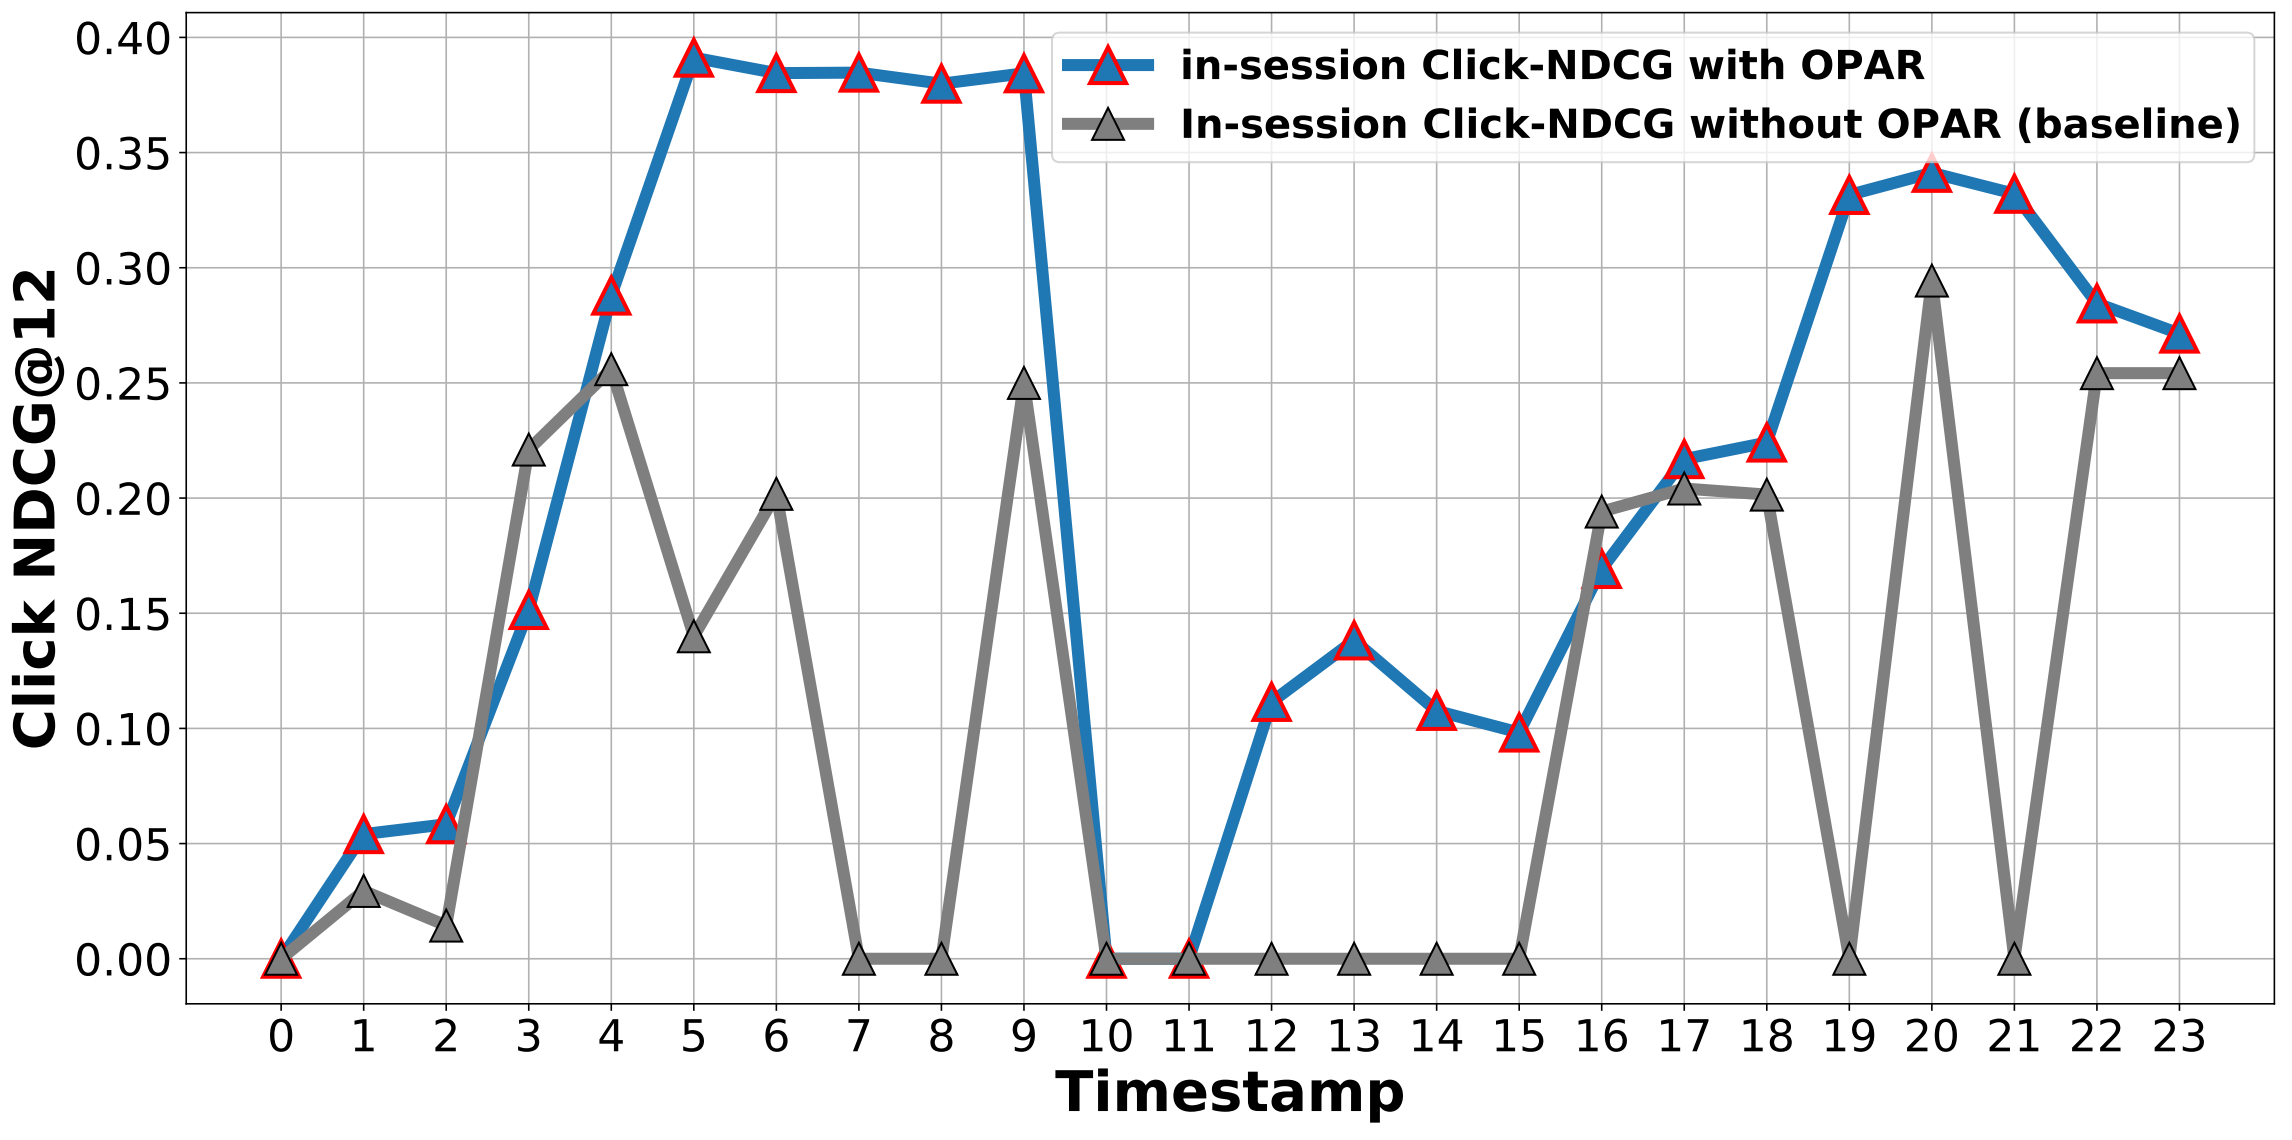
\includegraphics[bb=-200 0 0 60]{figs/Figure4_inSessionNDCG_png}
    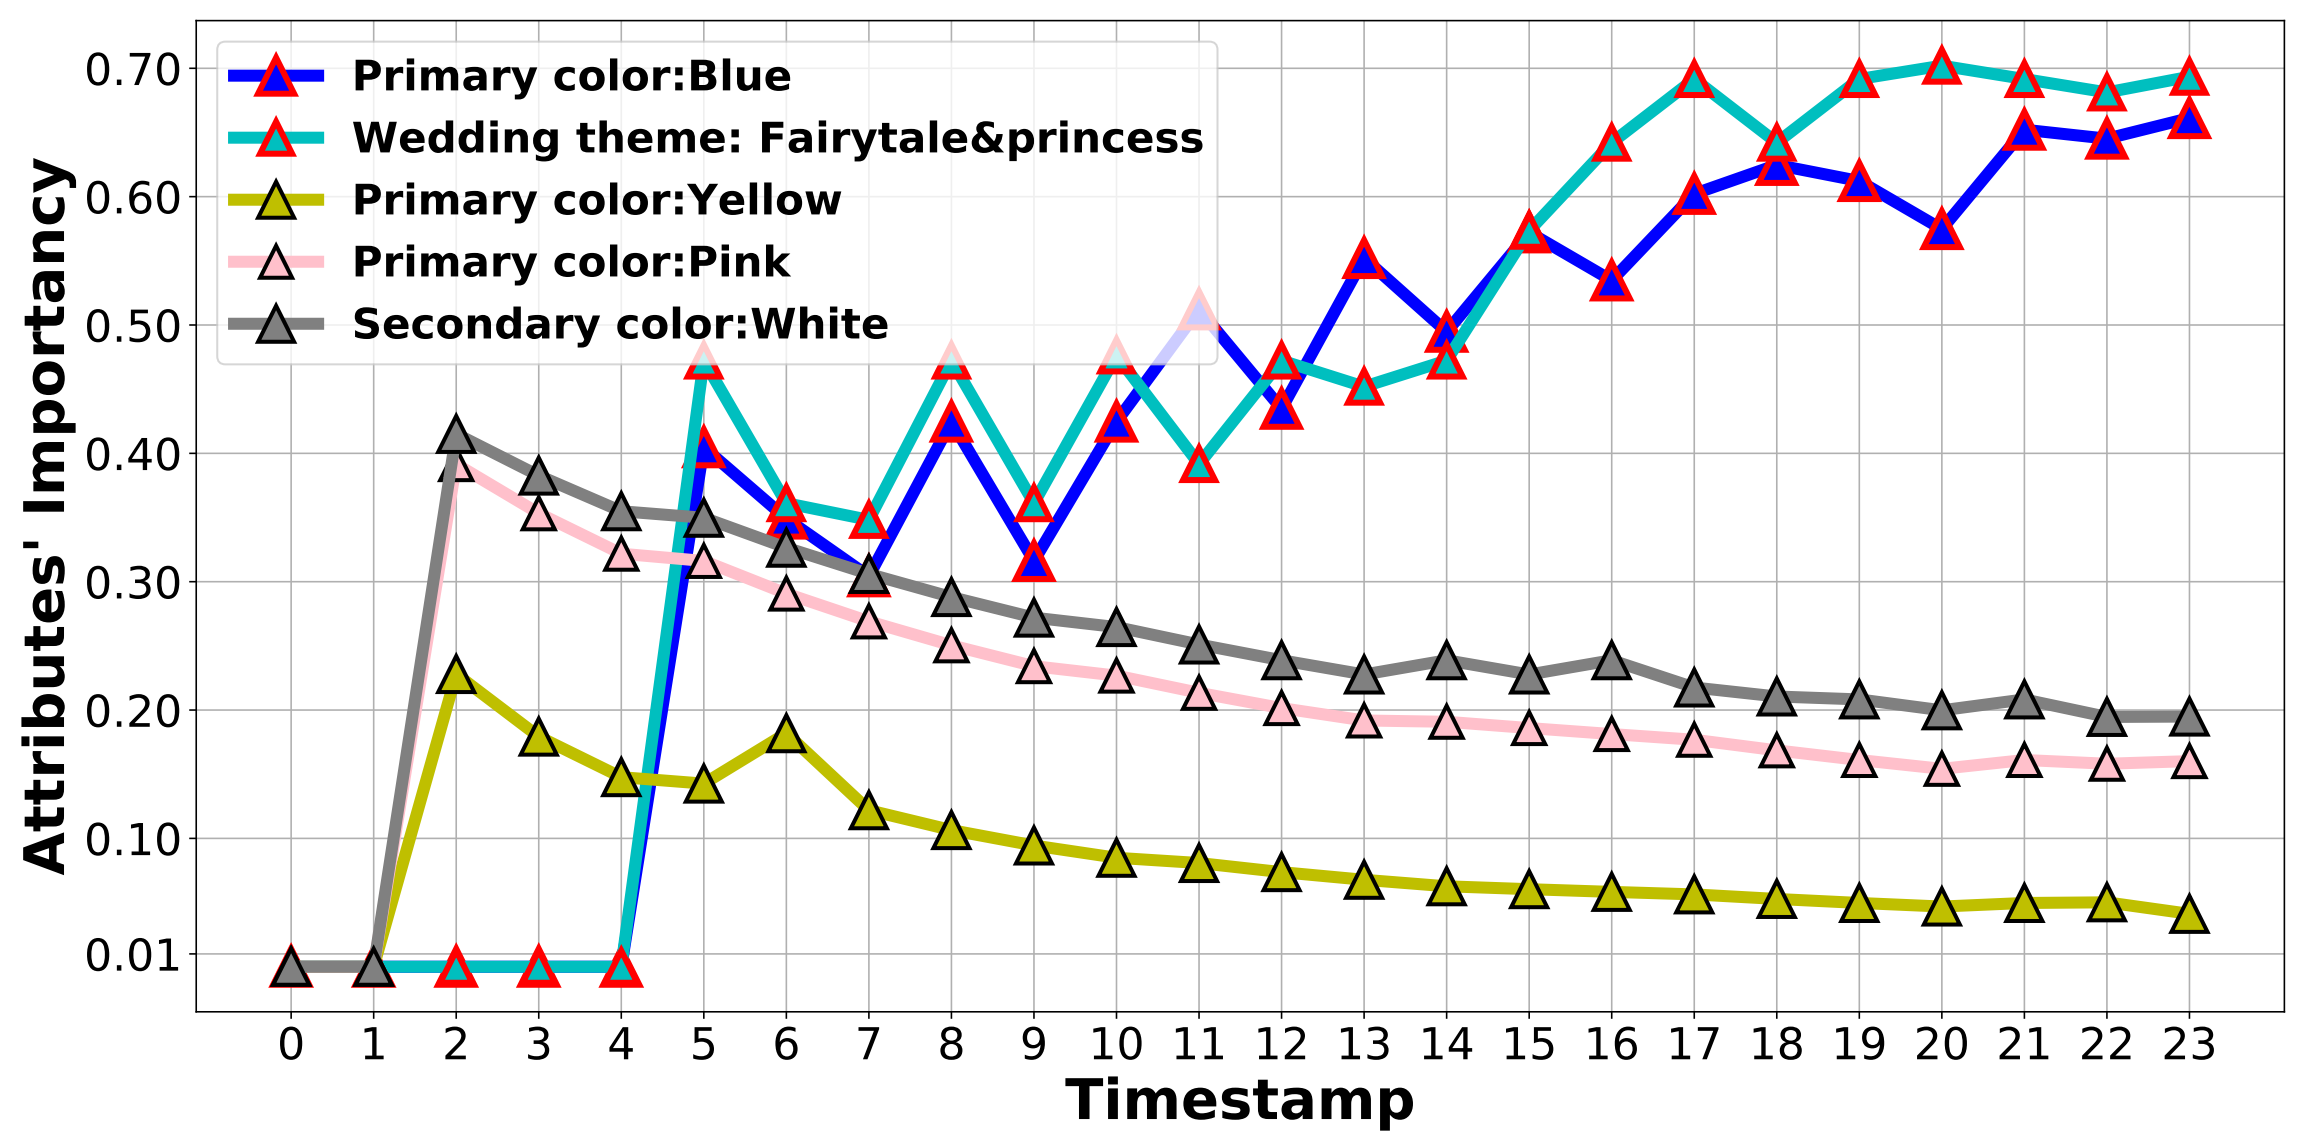
\includegraphics[bb=0 0 200 60]{figs/Figure5_interpretableAttribute_png}
    \caption{In-session \textit{OPAR} re-ranking performance.}
    \label{fig:multiIntent}
\end{figure}



%----------------------------------------------------------------------------------------------------------------------------------------------------------------
%--------------------------------------------------------------        SECTION 6       ---------------------------------------------------------------------
%----------------------------------------------------------------------------------------------------------------------------------------------------------------
\section{Conclusion}\label{sec:conclusion}
This paper proposes an interpretable \textit{Online Personalized Attributed-based Re-ranker (OPAR)} as a light-weight third-pass, followed by the normal 2-stage ranking process, to personalize a buyer's in-session experience based on product attributes. Given the important presence of attributes in the product category with its simplicity in explainability, we propose attribute-based multi-armed bandits to quickly learn the buyer's fine-grained preferences and re-rank items based on the recent activities within the session to achieve in-session personalization. We then extend the reward function of the attribute-based bandits to weight based on the type of actions the buyer interacts with the item (i.e, click, add-to-cart, purchase). Lastly, we train and evaluate \textit{OPAR} on the real-word e-commerce search ranking system, and show its superior performance against the baselines across multiples datasets. 
For future works, we could consider bias correction (i.e, position) in parameter updates to reduce self reinforcing, and model interactions between query and attributes to capture user preferences on attributes beyond engaged items. 


%----------------------------------------------------------------------------------------------------------------------------------------------------------------
%----------------------------------------------------------------------------------------------------------------------------------------------------------------
%----------------------------------------------------------------------------------------------------------------------------------------------------------------
\clearpage
\begin{thebibliography}{10}
\itemsep=1pt
\begin{small}

\bibitem{agrawal2012analysis} S.~Agrawal, N.~Goyal.
\newblock Analysis of thompson sampling for the multi-armed bandit problem.
\newblock Conference on learning theory, 2012.

\bibitem{Auer2002FinitetimeAO} P. Auer, N. Cesa-Bianchi, P. Fischer.
\newblock Finite-time Analysis of the Multiarmed Bandit Problem.
\newblock Machine Learning, 2002.


\bibitem{Auer2003EXP3} P.~Auer, N.~Cesa-Bianchi, Y.~Freund, R-E.~Schapire.
\newblock The Nonstochastic Multiarmed Bandit Problem.
\newblock Society for Industrial and Applied Mathematics, 2003.

\bibitem{sigir18_nextBucketRec} T.~Bai, Ting, J-Y.~Nie, W-X.~Zhao, Y.~Zhu, P.~Du, J-R.~Wen, Ji-Rong.
\newblock An Attribute-Aware Neural Attentive Model for Next Basket Recommendation.
\newblock The 41st International ACM SIGIR Conference on Research \& Development in Information Retrieval (SIGIR '18), 2018.
  
\bibitem{LDA} D-M.~Blei, A-Y.~Ng, M.I.~Jordan.
\newblock Latent Dirichlet Allocation.
\newblock Journal of Machine Learning Research, 2003.

\bibitem{burges2007learning} C-J.~Burges, R.~Ragno, Q-V.~Le.
\newblock Learning to rank with nonsmooth cost functions.
\newblock Advances in Neural Information Processing Systems, 2007.

\bibitem{NIPS2011_TS} C.~Olivier, L.~Li.
\newblock An Empirical Evaluation of Thompson Sampling.
\newblock Advances in Neural Information Processing Systems 24, 2011.

\bibitem{KDD19_streaming_sessionRecs} L.~Guo, H.~Yin, Q.~Wang, T.~Chen, A.~Zhou, N.~Quoc Viet Hung.
\newblock Streaming Session-Based Recommendation.
\newblock Proceedings of the 25th ACM SIGKDD International Conference on Knowledge Discovery and Data Mining, 2019.

\bibitem{guo2020debiasing} R.~Guo, X.~Zhao, A.~Henderson, L.~Hong, H.~Liu.
\newblock Debiasing Grid-based Product Search in E-commerce.
\newblock Proceedings of the 26th ACM SIGKDD International Conference on Knowledge Discovery \& Data Mining (KDD '20), 2020.

\bibitem{kdd20_DNN_airbnb_search} M.~Haldar, P.~Ramanathan, T.~Sax, M.~Abdool, L.~Zhang, A.~Mansawala, S.~Yang, B.~Turnbull, J.~Liao.
\newblock Improving Deep Learning for Airbnb Search.
\newblock Proceedings of the 26th ACM SIGKDD International Conference on Knowledge Discovery \& Data Mining (KDD '20), 2020.

\bibitem{Hidasi2016SessionbasedRW} B.~Hidasi, A.~Karatzoglou, L.~Baltrunas, D.~Tikk.
\newblock Session-based Recommendations with Recurrent Neural Networks.
\newblock arXiv: 1511.06939, 2015.

\bibitem{IJCAI17_sessionContextRecsys} L.~Hu, L.~Cao, S.~Wang, G.~Xu, J.~Cao, Z.~Gu.
\newblock Diversifying Personalized Recommendation with User-Session Context.
\newblock Proceedings of the 26th International Joint Conference on Artificial Intelligence (IJCAI’17), 2017.


\bibitem{KDD18_TaobaoSearch_RL} Y.~Hu, Q.~Da, A.~Zeng, Y.~Yu, Y.~Xu.
\newblock Reinforcement Learning to Rank in E-Commerce Search Engine: Formalization, Analysis, and Application.
\newblock Proceedings of the 24th ACM SIGKDD International Conference on Knowledge Discovery and Data Mining (KDD ’18), 2018.

\bibitem{kdd20_facebook_search} J-T.~Huang, A.~Sharma, S.~Sun, L.~Xia, D.~Zhang, P.~Pronin, J.~Padmanabhan, G.~Ottaviano, L.~Yang.
\newblock Embedding-Based Retrieval in Facebook Search. 
\newblock Proceddings of the 26th ACM SIGKDD International Conference on Knowledge Discovery \& Data Mining (KDD '20), 2020. 

\bibitem{li2017contextaware} L.~Shuai, K.~Purushottam.
\newblock Context-Aware Bandits.
\newblock arXiv: 1510.03164, 2015.

\bibitem{ICML16_contextCascadingBandits}
S.~Li, B.~Wang, S.~Zhang, W.~Chen, Wei.
\newblock Contextual Combinatorial Cascading Bandits.
\newblock Proceedings of the 33rd International Conference on International Conference on Machine Learning - Volume 48 (ICML'16), 2016.

\bibitem{KDD18_JD_nextItemRecs} Z.~Li,  H.~Zhao, Q.~Liu, Z.~Huang, T.~Mei, E.~Chen. \newblock Learning from History and Present: Next-Item Recommendation via Discriminatively Exploiting User Behaviors. \newblock Proceedings of the 24th ACM SIGKDD International Conference on Knowledge Discovery and Data Mining, 2018.

\bibitem{KDD18_STAMP} Q.~Liu, Y.~Zeng, R.~Mokhosi, H.~Zhang.
\newblock STAMP: Short-Term Attention/Memory Priority Model for Session-Based Recommendation. \newblock Proceedings of the 24th ACM SIGKDD International Conference on Knowledge Discovery and Data Mining, 2018.

\bibitem{liu2019convolution} X.~Liu, J.~He, S.~Duddy, L.~O'Sullivan, Liz.
\newblock Convolution-consistent collective matrix completion.
\newblock Proceedings of the 28th ACM international conference on information and knowledge management, p:2209--2212, 2019.

\bibitem{recsys17_userSesssionIntent} P.~Loyola, C.~Liu, Y.~Hirate.
\newblock Modeling User Session and Intent with an Attention-Based Encoder-Decoder Architecture. 
\newblock Proceedings of the Eleventh ACM Conference on Recommender Systems, 2017.

\bibitem{kdd19_amazon_product_search} P.~Nigam, Y.~Song, V.~Mohan, V.~Lakshman, W.~Ding, A.~Shingavi, H.~Teo, H.~Gu, B.~Yin. \newblock Semantic Product Search. \newblock Proceedings of the 25th ACM SIGKDD International Conference on Knowledge Discovery \& Data Mining, 2019.

\bibitem{pobrotyn2020contextaware} P.~Pobrotyn, T.~Bartczak, M.~Synowiec, R.~Białobrzeski, J.~Bojar.
\newblock Context-Aware Learning to Rank with Self-Attention. 
\newblock arXiv:2005.10084, 2020.

\bibitem{CIKM19_sessionRec_graphNN}
R.~Qiu, J.~Li, Z.~Huang, H.~Yin.
\newblock Rethinking the Item Order in Session-Based Recommendation with Graph Neural Networks.
\newblock Proceedings of the 28th ACM International Conference on Information and Knowledge Management (CIKM ’19), 2019.

\bibitem{recsys17_sessionRec_perso}
M.~Quadrana, A.~Karatzoglou, B.~Hidasi, P.~Cremonesi.
\newblock Personalizing Session-Based Recommendations with Hierarchical Recurrent Neural Networks.
\newblock Proceedings of the Eleventh ACM Conference on Recommender Systems (RecSys '17), 2017.

\bibitem{recsys19_interativeRecs} J.~Sanz-Cruzado, P.~Castells, E.~L\'{o}pez.
\newblock A Simple Multi-Armed Nearest-Neighbor Bandit for Interactive Recommendation.
\newblock RecSys, 2019. 

\bibitem{sutton2018reinforcement} R-S.~Sutton, A-G.~Barto, Andrew G.
\newblock Reinforcement learning: An introduction.
\newblock MIT press, 2018.

\bibitem{DLRS16_sessionBasedRecsys} Y-K.~Tan, X.~Xu, Y.~Liu.
\newblock Improved Recurrent Neural Networks for Session-Based Recommendations.
\newblock Proceedings of the 1st Workshop on Deep Learning for Recommender Systems (DLRS'16), 2016.

\bibitem{recsys16_amazon}
C-H.~Teo, H.~Nassif, D.~Hill, S.~Srinivasan, M.~Goodman, V.~Mohan, S-V-N.~Vishwanathan.
\newblock Adaptive, Personalized Diversity for Visual Discovery.
\newblock Proceedings of the 10th ACM Conference on Recommender Systems (RecSys '16), p:35–38, 2016.

\bibitem{IEEE19_onlineInterativeCF} Q.~Wang, C.~Zeng, W.~Zhou, T.~Li, S-S.~Iyengar, L.~Shwartz, G-Y.~Grabarnik.
\newblock Online Interactive Collaborative Filtering Using Multi-Armed Bandit with Dependent Arms.
\newblock IEEE Transactions on Knowledge and Data Engineering, 2019.

\bibitem{wang2013theoretical} Y.~Wang, L.~Wang, Y.~Li, D.~He, W.~Chen, T-Y.~Liu.
\newblock A theoretical analysis of NDCG ranking measures.
\newblock COLT: Proceedings of the 26th annual conference on learning theory, volume 8, page 6, 2013.

\bibitem{wu2018turning} L.~Wu, D.~Hu, L.~Hong, H.~Liu. \newblock Turning clicks into purchases: Revenue optimization for product search in e-commerce. \newblock The 41st International ACM SIGIR Conference on Research \& Development in Information Retrieval, 2018.

\bibitem{wu2010adapting} Q.~Wu, C.~Burges, S.~JC and K-M.~Svore, J.~Gao.
\newblock Adapting boosting for information retrieval measures.
\newblock Information Retrieval Journey, 2010.

\bibitem{MLKD19_JD_onlineRanking} Y.~Yan, Z.~Liu, M.~Zhao, W.~Guo, W-P.~Yan, Y.~Bao.
\newblock A practical deep online ranking system in e-commerce recommendation.
\newblock Springer: Joint European Conference on Machine Learning and Knowledge Discovery in Databases, p:186--201, 2018.

\bibitem{SIGIR16_RNN_nextBasketRec} F.~Yu, Q.~Liu, S.~Wu, L.~Wang, T.~Tan, Tieniu.
\newblock A Dynamic Recurrent Model for Next Basket Recommendation.
\newblock Proceedings of the 39th International ACM SIGIR Conference on Research and Development in Information Retrieval (SIGIR ’16), 2016.

\bibitem{2019_DNN_rec_survey} S.~Zhang, L.~Yao, A.~ Sun, Y.~Tay.
\newblock Deep Learning Based Recommender System: A Survey and New Perspectives.
\newblock ACM Comput. Surv., 2019.

\bibitem{elnlp2020_itemInteraction} X.~Zhao, R.~Louca, D.~Hu, L.~Hong. \newblock The Difference Between a Click and a Cart-Add: Learning Interaction-Specific Embeddings. \newblock Companion Proceedings of the Web Conference, 2020.

\bibitem{kdd20_sequentialRec} Y.~Zhao, Y-H.~Zhou, M.~Ou, H.~Xu, N.~Li. \newblock Maximizing Cumulative User Engagement in Sequential Recommendation: An Online Optimization Perspective. \newblock Proceedings of the 26th ACM SIGKDD International Conference on Knowledge Discovery \& Data Mining, 2020. 

\end{small}
\end{thebibliography}

\end{document}